\documentclass[11pt]{article}

\usepackage[margin=1in]{geometry}
\usepackage[T1]{fontenc}
\usepackage{lmodern}
\usepackage{microtype}
\usepackage{amsmath,amssymb,amsthm,mathtools}
\usepackage{booktabs,array,longtable,tabularx}
\usepackage{enumitem}
\usepackage{graphicx}
\usepackage{xcolor}
\usepackage{hyperref}
\usepackage{tikz}
\usetikzlibrary{arrows.meta,positioning,calc,fit,backgrounds,shapes.geometric}
\usepackage{pgfplots}
\pgfplotsset{compat=1.18}
\usepackage{caption}
\usepackage{subcaption}
\usepackage{fancyhdr}
\usepackage{lastpage}

\definecolor{accent}{RGB}{24,111,120}
\definecolor{accenttwo}{RGB}{58,76,132}
\definecolor{soft}{RGB}{240,246,247}
\definecolor{softtwo}{RGB}{242,243,249}
\definecolor{warn}{RGB}{145,72,70}

\hypersetup{
  colorlinks=true,
  linkcolor=accenttwo,
  urlcolor=accent,
  citecolor=accenttwo,
  pdftitle={Proof Compass Theory: Learnability, Shrinkage, and Control},
  pdfsubject={Technical report on theorem oceans, proof compasses, learning, pruning, fallback search, control theory, and Hodge-conjecture research next steps}
}

\pagestyle{fancy}
\fancyhf{}
\lhead{\small Proof Compass Theory}
\rhead{\small August 15, 2026}
\cfoot{\small \thepage\ of \pageref{LastPage}}

\newtheorem{theorem}{Theorem}[section]
\newtheorem{corollary}[theorem]{Corollary}
\newtheorem{proposition}[theorem]{Proposition}
\newtheorem{lemma}[theorem]{Lemma}
\newtheorem{conjecture}[theorem]{Conjecture}
\newtheorem{definition}[theorem]{Definition}
\newtheorem{remark}[theorem]{Remark}

\newcommand{\Prob}{\mathbb{P}}
\newcommand{\E}{\mathbb{E}}
\newcommand{\Ocal}{\mathcal{O}}
\newcommand{\Hcal}{\mathcal{H}}
\newcommand{\Dcal}{\mathcal{D}}
\newcommand{\Gcal}{\mathcal{G}}

\title{\textbf{Proof Compass Theory: Learnability, Shrinkage, and Control}\\
\large Technical Report on Theorem Oceans, Safe Pruning, Fallback Search, and Control-Theoretic Training}
\date{August 15, 2026}

\begin{document}

\begin{titlepage}
\centering
\vspace*{1.0in}
{\Huge\bfseries Proof Compass Theory\par}
\vspace{0.25in}
{\LARGE Learnability, Shrinkage, and Control\par}
\vspace{0.45in}
{\large A technical report on theorem oceans, proof compasses, safe pruning, fallback search, and control-theoretic training\par}
\vfill
{\large Prepared for Brian Tenneson\par}
\vspace{0.12in}
{\large August 15, 2026\par}
\vspace{0.4in}
\begin{minipage}{0.84\textwidth}
\small
\textbf{Status note.}
This report records the formalizations and synthetic experiments developed in the August 15, 2026 working session. Three broad conjectural claims are analyzed. Their unrestricted forms are not all true. Each admits a rigorous theorem under explicit hypotheses, and each theorem has operational corollaries relevant to automated theorem proving. The synthetic experiments are demonstrations of the mechanisms, not evidence that the corresponding claims already hold for the Hodge conjecture or for arbitrary ATP search.
\end{minipage}
\vfill
\end{titlepage}

\tableofcontents
\newpage

\section{Executive Summary}

The central object of this report is a \emph{proof compass}: a rule, learned or analytic, that assigns directional preference to proof-search states. The compass need not delete any mathematical objects. Its weakest use is to reorder the frontier. Its stronger use is to prune branches that are certified irrelevant. Its most useful robust form combines aggressive guidance with a complete fallback search.

Three conjectural ideas are studied.

\begin{enumerate}[label=\textbf{C\arabic*.},leftmargin=2.6em]
\item \textbf{Compass Learnability.} Solved proof DAGs can teach a compass that ranks useful successors above chance on unseen problems.
\item \textbf{Controlled Compass Shrinkage.} A learned compass can reduce effective proof-search cost while preserving eventual completeness through fallback.
\item \textbf{Adaptive Compass Control.} Control-theoretic selection of training examples can improve compass learning relative to passive or random training.
\end{enumerate}

The unrestricted form of C1 is false: if the visible proof state contains no information about the successful direction, no learner can recover a useful compass. A finite-class IID version with a positive population margin is proved by uniform convergence. C2 becomes a theorem under a simple cost-versus-survival condition: compass-first search with complete fallback improves expected cost whenever the probability that the restricted search retains a proof exceeds the restricted-ocean cost as a fraction of full-ocean cost. C3 becomes an exact one-step theorem in a linear-Gaussian model: choosing the next training state to maximize posterior trace reduction is optimal for that one-step uncertainty objective.

The experiments reproduce the predicted distinctions:
\begin{itemize}
\item informative IID data yield above-chance generalization with diminishing returns as training shells grow;
\item an uninformative representation returns chance performance;
\item severe distribution shift can produce an \emph{anti-compass};
\item hard pruning is fragile because local recall compounds along a proof;
\item a moderate beam width can outperform both narrow and exhaustive search when fallback is available;
\item active trace-reduction training learns substantially faster than random sampling in a deliberately redundant synthetic training ocean.
\end{itemize}

For current Hodge-conjecture work, the immediate recommendation is not to jump from these results to a claim about the global conjecture. Instead, the unresolved H2B1 finite-basis Hodge-star bridge should be converted into a controlled proof-compass testbed: quotient first, learn only from solved neighboring instances, instrument proof recall and fallback, and require verifier-checkable certificates before advancing the research ladder.

\section{Formal Setting and Definitions}

\subsection{Proof systems and theorem oceans}

\begin{definition}[Proof-search graph]
A proof-search graph is a directed graph
\[
G=(V,E)
\]
whose vertices are proof states and whose directed edges are legal proof-search transitions. A distinguished initial state is denoted \(v_0\). A set \(C\subseteq V\) contains certificate states: reaching any \(c\in C\) settles the target in the relevant direction.
\end{definition}

\begin{definition}[Bounded theorem ocean]
Given a resource or depth budget \(B\), the bounded theorem ocean is
\[
\Ocal_B(v_0)=\{v\in V:\text{\(v\) is reachable from \(v_0\) within budget \(B\)}\}.
\]
Its cardinality measures the number of proof states potentially encountered by a complete bounded search.
\end{definition}

The word ``ocean'' is deliberately broader than ``tree.'' Real proof search often merges equivalent states, reuses lemmas, and therefore forms a DAG or a general directed graph. A tree approximation is nevertheless useful for quantitative estimates.

\begin{definition}[Successor set]
For \(v\in V\),
\[
\Gamma(v)=\{u\in V:(v,u)\in E\}.
\]
\end{definition}

\begin{definition}[Proof path]
A proof path is a directed path
\[
v_0\to v_1\to\cdots\to v_d\in C.
\]
Its depth is \(d\).
\end{definition}

\subsection{Compass, ranking, pruning, and fallback}

\begin{definition}[Proof compass]
A proof compass is a measurable rule
\[
K:V\to \mathbb{R}^m
\]
or, more generally, a rule assigning a score or ordering to candidate successors. In the scalar case, larger \(K(u)\) means that successor \(u\) is searched earlier.
\end{definition}

\begin{definition}[Ranking compass]
A ranking compass changes only the order in which states are expanded. It leaves the reachable ocean unchanged.
\end{definition}

\begin{definition}[Pruning compass]
A pruning compass replaces \(\Gamma(v)\) by a retained set
\[
\Gamma_K(v)\subseteq \Gamma(v).
\]
\end{definition}

\begin{definition}[Safe pruning]
Pruning is safe for target set \(C\) if
\[
v\leadsto C
\quad\Longrightarrow\quad
\exists u\in\Gamma_K(v)\text{ with }u\leadsto C.
\]
Thus at least one successful continuation survives at every solvable state.
\end{definition}

\begin{definition}[Local proof recall]
For a learned top-\(k\) compass, local proof recall is
\[
q_k=\Prob(\text{at least one proof-successor appears among the top \(k\) ranked successors}).
\]
\end{definition}

\begin{definition}[Fallback search]
A fallback policy first searches a compass-restricted region and, if no certificate is found, returns to a complete baseline search. Fallback can preserve asymptotic completeness even when the learned compass is fallible.
\end{definition}

\begin{definition}[Effective branching factor]
When a policy retains or meaningfully explores an average of \(b_{\mathrm{eff}}\) successors per state, \(b_{\mathrm{eff}}\) is the effective branching factor. This is an operational quantity: it depends on the search policy, not merely on the formal proof system.
\end{definition}

\subsection{Solved DAGs and visible-state representations}

\begin{definition}[Solved proof DAG]
A solved proof DAG is a proof-search DAG together with at least one verified certificate path and enough retained search history to label local choices as more or less useful relative to a specified target.
\end{definition}

\begin{definition}[Visible-state representation]
A representation map
\[
\phi:V\to X
\]
specifies the information exposed to the learned compass. The representation may contain syntactic, semantic, proof-theoretic, geometric, historical, or resource-state features.
\end{definition}

A learned compass is a predictor \(h:X\to \mathbb{R}\) or \(h:X\times X\to\mathbb{R}\). Learnability is impossible if \(\phi(v)\) removes all information correlated with successful continuation.

\begin{figure}[ht]
\centering
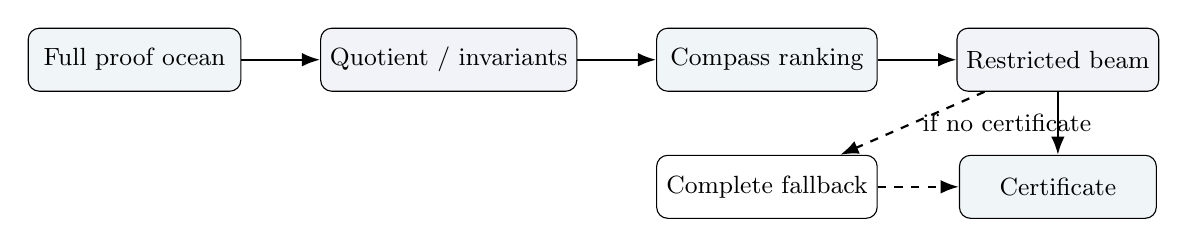
\begin{tikzpicture}[>=Latex, node distance=8mm and 10mm, every node/.style={font=\small}]
\node[draw,rounded corners,fill=soft,minimum width=2.7cm,minimum height=0.8cm] (ocean) {Full proof ocean};
\node[draw,rounded corners,fill=softtwo,right=of ocean,minimum width=2.9cm,minimum height=0.8cm] (quot) {Quotient / invariants};
\node[draw,rounded corners,fill=soft,right=of quot,minimum width=2.8cm,minimum height=0.8cm] (rank) {Compass ranking};
\node[draw,rounded corners,fill=softtwo,right=of rank,minimum width=2.5cm,minimum height=0.8cm] (beam) {Restricted beam};
\node[draw,rounded corners,fill=soft,below=of beam,minimum width=2.5cm,minimum height=0.8cm] (cert) {Certificate};
\node[draw,rounded corners,fill=white,below=of rank,minimum width=2.8cm,minimum height=0.8cm] (fallback) {Complete fallback};
\draw[->,thick] (ocean)--(quot);
\draw[->,thick] (quot)--(rank);
\draw[->,thick] (rank)--(beam);
\draw[->,thick] (beam)--(cert);
\draw[->,thick,dashed] (beam)--node[right]{if no certificate}(fallback);
\draw[->,thick,dashed] (fallback)--(cert);
\end{tikzpicture}
\caption{A robust compass architecture. Quotienting and certified invariants can shrink the formal ocean; ranking changes search order; a restricted beam changes the effective ocean; complete fallback protects completeness.}
\end{figure}

\section{Sufficient Conditions for Genuine Ocean Shrinkage}

\begin{theorem}[Safe Compass Shrinkage]
Let \(G=(V,E)\) be a proof-search graph with target set \(C\). Suppose a pruning compass satisfies:
\begin{enumerate}[label=(S\arabic*)]
\item for every \(v\) with \(v\leadsto C\), at least one retained successor \(u\in\Gamma_K(v)\) also satisfies \(u\leadsto C\);
\item \(|\Gamma_K(v)|\le k\) for every retained state, while the original branching is bounded by \(b\), with \(1\le k<b\).
\end{enumerate}
Then every proof path that exists from \(v_0\) has at least one proof-preserving counterpart in the compass-restricted graph. If all relevant proof depths are at most \(d\), then the restricted tree bound is
\[
1+k+\cdots+k^d
\]
instead of
\[
1+b+\cdots+b^d.
\]
\end{theorem}

\begin{proof}
If \(v_0\leadsto C\), condition (S1) gives a retained successor \(v_1\) that still reaches \(C\). Applying (S1) inductively produces a retained path until a certificate is reached. The node-count bounds follow from the branching assumptions.
\end{proof}

\begin{corollary}[Exponential reduction under uniform safe retention]
If the compass retains at most a fraction \(\rho\in(0,1)\) of the original successors at every level, so \(k\le \rho b\), then at depth \(d\) the leaf-count ratio is at most
\[
\left(\frac{k}{b}\right)^d\le \rho^d.
\]
Thus even modest safe local shrinkage compounds exponentially with depth.
\end{corollary}

\begin{definition}[Proof-search congruence]
An equivalence relation \(\sim\) on \(V\) is a proof-search congruence for target set \(C\) when
\[
v\sim w \Longrightarrow (v\leadsto C \iff w\leadsto C)
\]
and transitions descend consistently to equivalence classes.
\end{definition}

\begin{proposition}[Quotient-first shrinkage]
If \(\sim\) is a proof-search congruence, then complete search may be performed on \(V/{\sim}\) without losing target reachability.
\end{proposition}

\begin{corollary}[Multiplicative quotient-plus-compass reduction]
If the quotient reduces the relevant state count by a factor \(m>1\) on average and a safe compass subsequently reduces branching by a factor \(\rho<1\) over depth \(d\), then the combined leading-order reduction is approximately
\[
m^{-1}\rho^d
\]
relative to unquotiented blind search, subject to the graph structure and overlap assumptions used in the approximation.
\end{corollary}

This formalizes the operational principle
\[
\text{quotient first}\;\longrightarrow\;\text{compass second}\;\longrightarrow\;\text{fallback when needed}.
\]

\section{Conjecture I: Compass Learnability}

\subsection{Broad conjecture and denial without signal}

\begin{conjecture}[Broad Compass Learnability Conjecture]
For suitable families of proof-search problems and sufficiently informative visible-state representations, training on retained solved DAGs yields a predictor whose local tunnel-ranking accuracy on unseen problems is substantially above chance.
\end{conjecture}

The words ``suitable,'' ``informative,'' and ``substantially'' hide the necessary assumptions. Without them, the corresponding universal claim is false.

\begin{proposition}[No-signal impossibility]
Let \(X\) be the visible state and \(Y\) the identity of a successful successor. If \(X\) and \(Y\) are independent and the \(b\) successor labels are equiprobable, then no decision rule based only on \(X\) can achieve expected top-1 accuracy above \(1/b\) or top-\(k\) recall above \(k/b\).
\end{proposition}

\begin{proof}
Independence gives \(\Prob(Y=j\mid X)=\Prob(Y=j)=1/b\). Therefore no function of \(X\) can change the posterior distribution over \(Y\). The optimal top-\(k\) set captures exactly \(k/b\) probability mass.
\end{proof}

\begin{corollary}[Representation is a necessary research variable]
If a compass experiment remains at chance despite increasing training size, one cannot conclude merely that the learning algorithm is weak. The visible-state representation itself may have zero or negligible predictive information about proof continuation.
\end{corollary}

\subsection{A theorem under explicit hypotheses}

For a solved DAG \(G\), let \(A_G(h)\in[0,1]\) be the local pairwise ranking accuracy of compass \(h\). Let
\[
A(h)=\E_{G\sim\Dcal}[A_G(h)].
\]

\begin{theorem}[Finite-Class Compass Learnability]
Assume:
\begin{enumerate}[label=(L\arabic*)]
\item \(G_1,\ldots,G_N,G_{\mathrm{test}}\) are IID draws from a fixed distribution \(\Dcal\);
\item the hypothesis class \(\Hcal\) is finite;
\item there exists \(h^\star\in\Hcal\) such that
\[
A(h^\star)\ge \frac12+2\gamma
\]
for some \(\gamma>0\);
\item the learned compass is an empirical maximizer
\[
\widehat h\in\arg\max_{h\in\Hcal}\frac1N\sum_{i=1}^N A_{G_i}(h).
\]
\end{enumerate}
If
\[
N\ge \frac{2}{\gamma^2}\log\frac{2|\Hcal|}{\delta},
\]
then, with probability at least \(1-\delta\),
\[
A(\widehat h)\ge \frac12+\gamma.
\]
\end{theorem}

\begin{proof}
For any fixed \(h\), Hoeffding's inequality gives
\[
\Prob\bigl(|\widehat A(h)-A(h)|>\epsilon\bigr)\le 2e^{-2N\epsilon^2}.
\]
A union bound over \(\Hcal\) gives
\[
\Prob\left(\sup_{h\in\Hcal}|\widehat A(h)-A(h)|>\epsilon\right)
\le 2|\Hcal|e^{-2N\epsilon^2}.
\]
Set \(\epsilon=\gamma/2\). Under the stated sample-size bound, the event of uniform deviation greater than \(\gamma/2\) has probability at most \(\delta\). On its complement,
\[
A(\widehat h)
\ge \widehat A(\widehat h)-\frac{\gamma}{2}
\ge \widehat A(h^\star)-\frac{\gamma}{2}
\ge A(h^\star)-\gamma
\ge \frac12+\gamma.
\]
\end{proof}

\begin{corollary}[Sample complexity and shell design]
For fixed \(\delta\) and model complexity, the number of solved DAGs required to certify a target advantage \(\gamma\) scales as \(O(\gamma^{-2})\). Consequently, doubling the training shell does not generally double generalization quality; diminishing marginal improvements are expected once estimation error is no longer dominant.
\end{corollary}

\begin{corollary}[Distribution shift can invalidate the theorem]
The theorem gives no guarantee if unseen problems are not drawn from the training distribution. A compass may therefore require explicit distribution-shift diagnostics or bounded intervention policies before it is trusted for pruning.
\end{corollary}

\subsection{Synthetic shell experiment}

A synthetic proof family was constructed with \(b=12\) successors per state and an 8-dimensional hidden linear progress direction. A solved state supplies a noisy progress label. Ridge regression learns the compass. The test family is IID unless explicitly changed.

\begin{table}[ht]
\centering
\caption{Synthetic compass learning as the training shell grows. Chance top-1 is \(1/12\approx0.0833\); chance top-3 is \(3/12=0.25\).}
\begin{tabular}{rrrrr}
\toprule
Training \(N\) & Top-1 & Top-3 & Pairwise accuracy & Mean proof rank\\
\midrule
10  & 0.3959 & 0.7167 & 0.8289 & 2.8819\\
20  & 0.4655 & 0.7951 & 0.8731 & 2.3964\\
40  & 0.5189 & 0.8441 & 0.9000 & 2.1004\\
80  & 0.5446 & 0.8658 & 0.9103 & 1.9862\\
160 & 0.5559 & 0.8740 & 0.9147 & 1.9386\\
320 & 0.5604 & 0.8761 & 0.9160 & 1.9237\\
\bottomrule
\end{tabular}
\end{table}

\begin{figure}[ht]
\centering
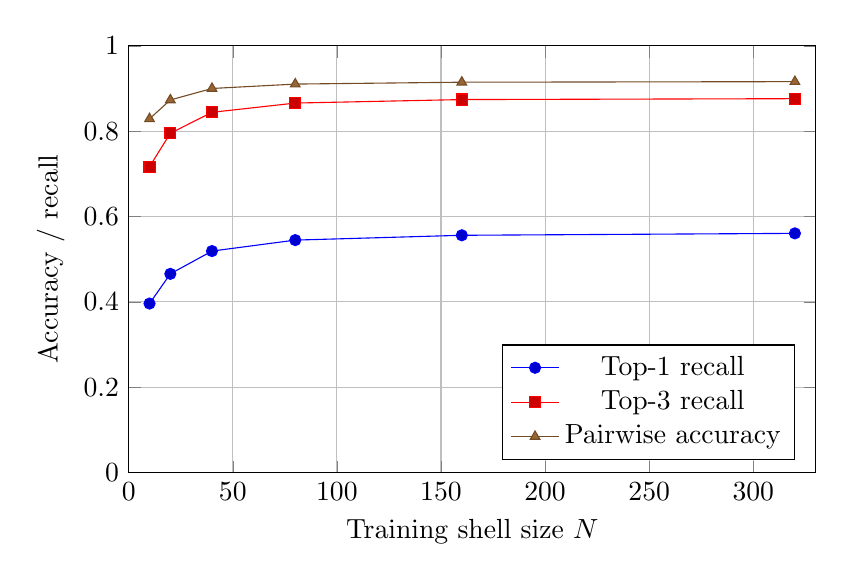
\begin{tikzpicture}
\begin{axis}[
width=.85\textwidth,
height=7cm,
xlabel={Training shell size \(N\)},
ylabel={Accuracy / recall},
xmin=0,xmax=330,
ymin=0,ymax=1,
grid=both,
legend pos=south east,
]
\addplot+[mark=*] coordinates {(10,.3959)(20,.4655)(40,.5189)(80,.5446)(160,.5559)(320,.5604)};
\addlegendentry{Top-1 recall}
\addplot+[mark=square*] coordinates {(10,.7167)(20,.7951)(40,.8441)(80,.8658)(160,.8740)(320,.8761)};
\addlegendentry{Top-3 recall}
\addplot+[mark=triangle*] coordinates {(10,.8289)(20,.8731)(40,.9000)(80,.9103)(160,.9147)(320,.9160)};
\addlegendentry{Pairwise accuracy}
\end{axis}
\end{tikzpicture}
\caption{The synthetic informative family exhibits strong early learning and diminishing returns.}
\end{figure}

\subsection{Counterexamples by experiment}

With \(N=160\), three test regimes were compared.

\begin{table}[ht]
\centering
\caption{The same trained compass under IID testing, no-signal testing, and a severe sign-reversing distribution shift.}
\begin{tabularx}{\textwidth}{Xrrrr}
\toprule
Scenario & Top-1 & Top-3 & Pairwise & Mean rank\\
\midrule
IID informative test & 0.5552 & 0.8697 & 0.9135 & 1.9516\\
Uninformative visible state & 0.0864 & 0.2514 & 0.5017 & 6.4817\\
Distribution shift: test direction is opposite training direction & 0.0001 & 0.0015 & 0.0863 & 11.0502\\
\bottomrule
\end{tabularx}
\end{table}

The third row is especially important: a compass that learned real structure became an \emph{anti-compass} under severe shift. Robust search should therefore treat learned guidance as a fallible control signal rather than as an oracle.

\section{Conjecture II: Controlled Compass Shrinkage}

\begin{conjecture}[Controlled Compass Shrinkage Conjecture]
For sufficiently structured proof families, a learned compass combined with bounded pruning and complete fallback can lower expected certificate-hitting cost on unseen problems relative to immediate exhaustive search.
\end{conjecture}

The general phrase ``sufficiently structured'' remains broad. A precise sufficient condition follows.

\begin{theorem}[Fallback Compass Advantage]
Let \(C_b\) be the cost of the complete baseline search, \(C_k\) the cost of searching a compass-restricted region first, and
\[
Q=\Prob(\text{the restricted region contains a proof}).
\]
Consider the policy: search the restricted region; if it fails, run the complete baseline search. Then
\[
\E[T]\le C_k+(1-Q)C_b.
\]
In particular,
\[
\E[T]<C_b
\]
whenever
\[
Q>\frac{C_k}{C_b}.
\]
\end{theorem}

\begin{proof}
If the restricted region contains a proof, the policy costs at most \(C_k\). If it does not, the policy costs at most \(C_k+C_b\). Therefore
\[
\E[T]\le Q C_k+(1-Q)(C_k+C_b)
= C_k+(1-Q)C_b.
\]
The strict advantage condition is equivalent to
\[
C_k+(1-Q)C_b<C_b,
\]
which rearranges to \(Q>C_k/C_b\).
\end{proof}

\begin{corollary}[Beam-width survival condition]
Suppose a unique successful continuation must survive \(d\) approximately independent local compass decisions, each with top-\(k\) recall \(q_k\). Then
\[
Q\approx q_k^d.
\]
A sufficient condition for expected advantage is
\[
q_k^d>\frac{C_k}{C_b}.
\]
\end{corollary}

\begin{corollary}[Existence of an optimal finite beam width]
If \(k\in\{1,\ldots,b\}\) and \(q_k\) is empirically estimable, then the conservative objective
\[
J(k)=\frac{C_k}{C_b}+1-q_k^d
\]
has at least one minimizer \(k^\star\). Thus beam width can be treated as a control variable rather than a fixed architectural constant.
\end{corollary}

\begin{remark}
High local accuracy does not imply safe hard pruning. For example, \(q=0.95\) over \(100\) independent required decisions gives survival \(0.95^{100}\approx0.0059\). The multiplicative recall effect is the central reason to prefer fallback over irreversible learned deletion.
\end{remark}

\subsection{Synthetic beam-width experiment}

Using \(b=12\), depth \(d=7\), and a compass trained on \(N=40\) observations, the top-\(k\) beam was searched first and complete fallback was charged upon failure.

\begin{table}[ht]
\centering
\caption{Selected beam widths. The final column is the conservative expected-cost upper bound relative to full search.}
\begin{tabular}{rrrrr}
\toprule
\(k\) & Local recall \(q_k\) & Path survival & Restricted/full cost & Expected-cost ratio\\
\midrule
1 & 0.53722 & 0.01291 & 0.00000 & 0.98709\\
3 & 0.86214 & 0.35403 & 0.00008 & 0.64605\\
5 & 0.95656 & 0.73280 & 0.00250 & 0.26970\\
6 & 0.97702 & 0.84981 & 0.00859 & 0.15878\\
7 & 0.98824 & 0.92053 & 0.02458 & 0.10405\\
8 & 0.99496 & 0.96525 & 0.06131 & 0.09607\\
9 & 0.99818 & 0.98733 & 0.13766 & 0.15033\\
12& 1.00000 & 1.00000 & 1.00000 & 1.00000\\
\bottomrule
\end{tabular}
\end{table}

The best tested width was \(k=8\), not the narrowest beam. It retained two thirds of local successors, yet the depth-seven restricted ocean was only about \(6.1\%\) of the full tree while the proof survived about \(96.5\%\) of the time. The conservative bound corresponded to an expected-cost ratio of approximately \(0.096\), or a lower-bound speedup of about \(10.4\) in this synthetic model.

\begin{figure}[ht]
\centering
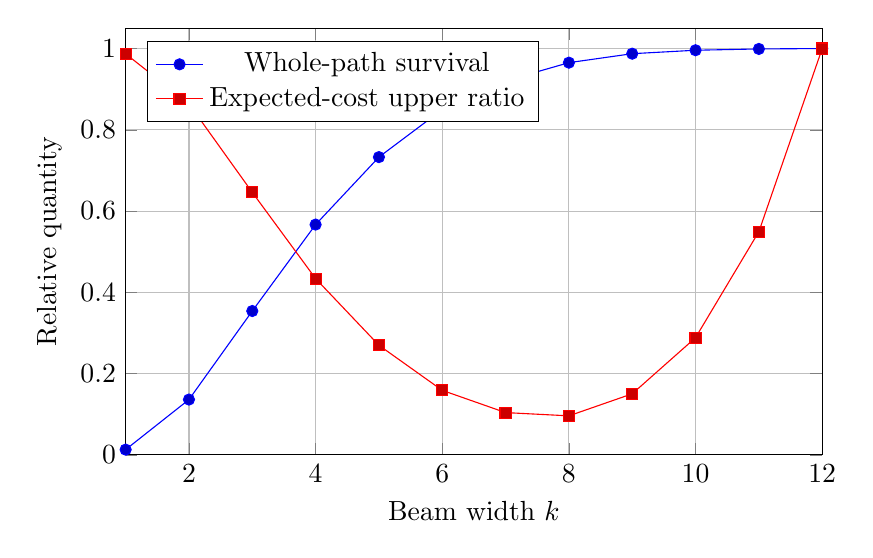
\begin{tikzpicture}
\begin{axis}[
width=.86\textwidth,
height=7cm,
xlabel={Beam width \(k\)},
ylabel={Relative quantity},
xmin=1,xmax=12,
ymin=0,ymax=1.05,
grid=both,
legend pos=north west,
]
\addplot+[mark=*] coordinates {
(1,.01291)(2,.13612)(3,.35403)(4,.56674)(5,.73280)(6,.84981)
(7,.92053)(8,.96525)(9,.98733)(10,.99581)(11,.99902)(12,1.0)};
\addlegendentry{Whole-path survival}
\addplot+[mark=square*] coordinates {
(1,.98709)(2,.86388)(3,.64605)(4,.43382)(5,.26970)(6,.15878)
(7,.10405)(8,.09607)(9,.15033)(10,.28844)(11,.54936)(12,1.0)};
\addlegendentry{Expected-cost upper ratio}
\end{axis}
\end{tikzpicture}
\caption{The optimal beam is a compromise: too narrow loses proofs; too wide keeps too much ocean.}
\end{figure}

\section{Conjecture III: Adaptive Compass Control}

\begin{conjecture}[Adaptive Compass Control Conjecture]
For practically relevant theorem families, feedback control over training-example selection, curriculum, beam width, uncertainty, and fallback can reduce expected certificate-hitting time on unseen problems relative to random training and a fixed compass policy.
\end{conjecture}

This remains open in its full nonlinear, nonstationary form. A precise one-step version is provable.

\subsection{Linear-Gaussian control theorem}

Assume a hidden compass parameter \(w\in\mathbb{R}^p\) and observations
\[
y=x^\top w+\epsilon,\qquad \epsilon\sim N(0,\sigma^2).
\]
Let the current posterior be
\[
w\mid D_t\sim N(m_t,P_t).
\]
After observing candidate \(x\), the posterior covariance is
\[
P_{t+1}
=
P_t-
\frac{P_txx^\top P_t}{\sigma^2+x^\top P_tx}.
\]

\begin{theorem}[One-Step Trace-Optimal Compass Training]
If uncertainty is measured by \(V(P)=\operatorname{tr}(P)\), then the one-step reduction in posterior uncertainty obtained by sampling \(x\) is
\[
\Delta(x)
=
\frac{x^\top P_t^2x}{\sigma^2+x^\top P_tx}.
\]
Therefore the control law
\[
x_t^\star
\in
\arg\max_x
\frac{x^\top P_t^2x}{\sigma^2+x^\top P_tx}
\]
maximizes the one-step reduction in posterior trace uncertainty among the available candidates.
\end{theorem}

\begin{proof}
Take the trace of the covariance update:
\[
\operatorname{tr}(P_t)-\operatorname{tr}(P_{t+1})
=
\operatorname{tr}\left(
\frac{P_txx^\top P_t}{\sigma^2+x^\top P_tx}
\right).
\]
Using cyclicity of trace,
\[
\operatorname{tr}(P_txx^\top P_t)=x^\top P_t^2x.
\]
The result follows.
\end{proof}

\begin{corollary}[One-step active dominance over random sampling]
Let a random policy draw a candidate \(X\) from a finite available set. Then
\[
\E[\Delta(X)]\le \max_x\Delta(x).
\]
If the random policy gives positive probability to any candidate with strictly smaller \(\Delta\) than the maximum, the inequality is strict. Hence the trace-optimal controller weakly dominates random sampling for the one-step uncertainty objective and strictly dominates it whenever the candidate information gains are nonuniform.
\end{corollary}

\begin{corollary}[Control cannot create missing information]
If every available candidate satisfies \(x^\top P_t^2x=0\), then \(\Delta(x)=0\) for every control action. No training scheduler can reduce uncertainty along directions that are completely unobservable in the candidate pool.
\end{corollary}

\subsection{Synthetic control experiment}

A deliberately redundant candidate pool was generated so that random training repeatedly oversampled a small part of parameter space. The active policy selected the candidate maximizing one-step trace reduction.

\begin{table}[ht]
\centering
\caption{Random versus actively controlled compass training.}
\begin{tabular}{rllrr}
\toprule
Observations & Curriculum & \(\operatorname{tr}(P)\) & Parameter MSE & Top-3 recall\\
\midrule
5  & random & 4.7245 & 4.8219 & 0.6032\\
5  & active & 3.5537 & 3.7358 & 0.6679\\
10 & random & 3.1030 & 3.1869 & 0.7016\\
10 & active & 0.7758 & 0.8449 & 0.8459\\
20 & random & 1.6357 & 1.6217 & 0.8004\\
20 & active & 0.3824 & 0.3736 & 0.8757\\
40 & random & 0.6964 & 0.7099 & 0.8540\\
40 & active & 0.1924 & 0.1986 & 0.8850\\
80 & random & 0.2930 & 0.2814 & 0.8812\\
80 & active & 0.0970 & 0.0989 & 0.8911\\
\bottomrule
\end{tabular}
\end{table}

At ten observations, active control reduced posterior trace from \(3.1030\) to \(0.7758\) and increased top-3 recall from \(0.7016\) to \(0.8459\). The gap narrows as both methods approach the information ceiling of the synthetic model, again showing diminishing returns.

\section{A Unified Compass-Control Architecture}

The three results can be assembled into a single closed-loop architecture.

\begin{figure}[ht]
\centering
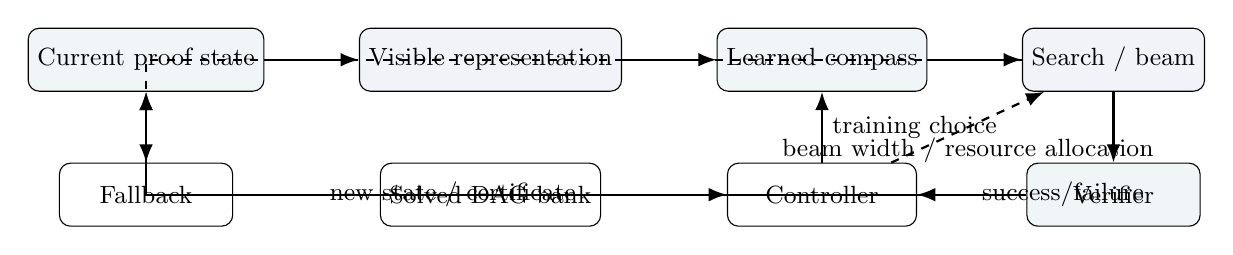
\begin{tikzpicture}[>=Latex, node distance=9mm and 12mm, every node/.style={font=\small}]
\node[draw,rounded corners,fill=soft,minimum width=2.6cm,minimum height=.8cm] (problem) {Current proof state};
\node[draw,rounded corners,fill=softtwo,right=of problem,minimum width=2.6cm,minimum height=.8cm] (repr) {Visible representation};
\node[draw,rounded corners,fill=soft,right=of repr,minimum width=2.3cm,minimum height=.8cm] (compass) {Learned compass};
\node[draw,rounded corners,fill=softtwo,right=of compass,minimum width=2.2cm,minimum height=.8cm] (search) {Search / beam};
\node[draw,rounded corners,fill=soft,below=of search,minimum width=2.2cm,minimum height=.8cm] (verify) {Verifier};
\node[draw,rounded corners,fill=white,below=of compass,minimum width=2.4cm,minimum height=.8cm] (controller) {Controller};
\node[draw,rounded corners,fill=white,below=of repr,minimum width=2.4cm,minimum height=.8cm] (bank) {Solved DAG bank};
\node[draw,rounded corners,fill=white,below=of problem,minimum width=2.2cm,minimum height=.8cm] (fallback) {Fallback};
\draw[->,thick] (problem)--(repr);
\draw[->,thick] (repr)--(compass);
\draw[->,thick] (compass)--(search);
\draw[->,thick] (search)--(verify);
\draw[->,thick] (verify.west) -| node[pos=.25,left]{new state / certificate} (problem.south);
\draw[->,thick] (bank)--(controller);
\draw[->,thick] (controller)--node[right]{training choice}(compass);
\draw[->,thick] (verify)--node[right]{success/failure}(controller);
\draw[->,thick,dashed] (controller)--node[below]{beam width / resource allocation}(search);
\draw[->,thick,dashed] (search.west) -| (fallback.north);
\draw[->,thick,dashed] (fallback)--(problem);
\end{tikzpicture}
\caption{Closed-loop proof-compass control. The controller acts both on learning and on search width, while the verifier anchors correctness and fallback limits the cost of compass error.}
\end{figure}

A natural objective is not merely ranking accuracy. It is closer to
\[
J=
\E[T_{\mathrm{certificate}}]
+\lambda\,\Prob(\mathrm{fallback})
+\mu\,C_{\mathrm{training}}
+\nu\,C_{\mathrm{unsafe\ pruning}},
\]
with the last term taken as infinite if certificate-preserving guarantees are mandatory.

The architecture suggests four distinct uncertainty channels:
\begin{enumerate}
\item \textbf{epistemic uncertainty}: uncertainty in the learned compass;
\item \textbf{distribution uncertainty}: uncertainty that the current problem belongs to the learned family;
\item \textbf{search uncertainty}: uncertainty about the remaining proof depth and branching;
\item \textbf{verification uncertainty}: uncertainty removed only by formal certificate checking.
\end{enumerate}

These should not be conflated. In particular, high compass confidence does not imply in-distribution status, and in-distribution status does not imply safe pruning.

\section{Implications for the Hodge-Conjecture Program}

\subsection{Current position}

The current Hodge program has verified H0 and H1 substrates and has banked several H2 nodes. The active mathematical bottleneck is the finite basis-level Hodge-star bridge, designated H2B1. Recent quotient-first and certificate-recovery attempts, including the strict next-rung sweep, did not settle H2B1. Therefore the correct use of the present compass results is methodological: redesign the H2B1 search so that guidance, pruning, and fallback are explicitly measurable.

\subsection{Recommended next steps}

\paragraph{1. Freeze H2B1 as a benchmark before changing the search.}
Specify the exact premises, target statement, admissible transformations, verifier, resource budget, and success certificate. The objective is to prevent changes in representation or search policy from silently changing the theorem being tested.

\paragraph{2. Separate quotienting from learning.}
Before training a compass, define as many proof-search congruences as can be justified exactly: syntactic symmetries, basis relabelings, equivalent linear/bilinear forms, duplicated normal forms, and any verified Hodge-star identities that preserve target reachability. Measure the quotient factor independently of any learned model.

\paragraph{3. Build a bank of solved neighboring DAGs.}
Do not train directly on the unresolved target alone. Generate or retain solved finite-basis neighbors: smaller dimensions, restricted coefficient families, linear subcases, bilinear subcases, symmetry-reduced instances, and already banked H2 lemmas. Each solved DAG should retain successful and unsuccessful local choices so that ranking labels are not trivial.

\paragraph{4. Define Hodge-specific visible-state features.}
Candidate features should include proof depth, unsatisfied subgoals, normal-form signatures, Hodge-type bookkeeping, linear/bilinear rank information, symmetry class, lemma-bank overlap, Hodge-star compatibility tests, and verifier-derived obstruction flags. A feature should be included because it could carry information about future proof success, not merely because it is easy to compute.

\paragraph{5. Run shell learnability tests.}
Use fixed nested training shells such as \(10,20,40,80\) solved DAGs, holding the unseen H2B1-like test family fixed. Record top-\(k\) proof recall, pairwise ranking accuracy, mean proof-successor rank, effective branching factor, certificate-hitting time, and fallback frequency.

\paragraph{6. Add explicit distribution-shift controls.}
Train on one restricted family and test on a deliberately shifted family. The purpose is to determine whether the Hodge compass degrades gracefully or becomes an anti-compass. No hard learned pruning should be allowed until this behavior is understood.

\paragraph{7. Optimize beam width by measured recall, not taste.}
Estimate \(q_k\) on held-out solved DAGs and evaluate
\[
J(k)=\frac{C_k}{C_b}+1-q_k^d
\]
or a directly measured analog. Let the controller choose \(k\) adaptively from uncertainty and shift diagnostics.

\paragraph{8. Preserve a complete verifier-anchored fallback.}
The compass may decide where to search first, but it should not be allowed to convert uncertainty into a false mathematical conclusion. If the restricted search fails, the baseline search remains available. All claimed H2B1 progress must end in verifier-checkable lemmas or certificates.

\paragraph{9. Test controlled curriculum selection.}
Compare at least four regimes:
\begin{enumerate}
\item no compass;
\item compass trained on random solved neighbors;
\item compass trained by uncertainty/diversity control;
\item quotient-first plus controlled compass plus fallback.
\end{enumerate}
The experimental question is whether control buys actual certificate time, not merely better classification scores.

\paragraph{10. Advance the Hodge ladder only on a predeclared criterion.}
A reasonable next-rung criterion is: H2B1 is considered advanced only when a verifier-checkable certificate or lemma is produced that survives an independent rerun and whose use does not depend on hidden target leakage from the solved training set.

\subsection{A Hodge-specific open conjecture for later work}

\begin{conjecture}[Hodge Local-Transfer Compass Conjecture]
There exists a family of finite-basis Hodge-star bridge problems surrounding H2B1 and a target-independent visible-state representation for which a compass trained on solved neighboring DAGs achieves held-out top-\(k\) proof recall above chance and reduces expected verifier-certified hitting time under complete fallback.
\end{conjecture}

This conjecture is deliberately local. It does not imply the Hodge conjecture. Its purpose is to decide whether proof-compass methods are relevant to the current rung at all.

\begin{corollary}[Operational meaning of a positive local-transfer result]
If the Hodge Local-Transfer Compass Conjecture holds with measured survival probability \(Q\) and restricted/full cost ratio \(C_k/C_b\) satisfying
\[
Q>C_k/C_b,
\]
then the fallback advantage theorem predicts a genuine expected search-time advantage on that benchmark family, even though no claim about the global Hodge conjecture follows.
\end{corollary}

\section{Experimental Protocol for a Real ATP Implementation}

A clean implementation should log one row per proof-state decision with:
\begin{itemize}
\item problem identifier and family;
\item training-shell membership;
\item visible-state feature hash;
\item successor set size;
\item compass scores and ranks;
\item whether each successor is known, retrospectively, to lie on a retained successful DAG;
\item chosen beam width;
\item whether fallback was triggered;
\item verifier status;
\item cumulative expansions, wall time, and memory;
\item certificate identifier if settlement occurs.
\end{itemize}

The primary outcome variables should be:
\[
(q_1,q_3,q_5,\ldots),\quad
b_{\mathrm{eff}},\quad
T_{\mathrm{certificate}},\quad
\Prob(\mathrm{fallback}),
\]
together with distribution-shift diagnostics.

Ablations should isolate the contribution of each component:
\[
\text{quotient},\quad
\text{compass},\quad
\text{adaptive beam},\quad
\text{controlled curriculum},\quad
\text{fallback}.
\]

\section{What Has Been Settled and What Remains Open}

\begin{longtable}{p{0.28\textwidth}p{0.23\textwidth}p{0.41\textwidth}}
\toprule
Claim & Status & Precise interpretation\\
\midrule
\endfirsthead
\toprule
Claim & Status & Precise interpretation\\
\midrule
\endhead
Safe compass shrinkage & Proved & If at least one proof-preserving successor is retained at every solvable state, the target remains reachable and branching can shrink.\\
Broad universal compass learnability & Denied & False when the visible state carries no information about the successful direction.\\
Finite-class compass learnability & Proved under hypotheses & IID data, positive population margin, finite hypothesis class, and enough solved DAGs imply above-chance unseen ranking.\\
Hard learned pruning is safe whenever local accuracy is high & Denied & Local recall compounds multiplicatively along long proofs.\\
Fallback compass advantage & Proved & Expected cost improves when proof-survival probability exceeds restricted/full search-cost ratio.\\
A fixed narrow beam is always best & Denied experimentally & In the synthetic test, a moderate beam was better than both very narrow and exhaustive beams.\\
One-step control can maximize compass learning & Proved in linear-Gaussian trace model & The information-maximizing candidate has a closed-form acquisition score.\\
General adaptive compass control & Open & Nonlinear, nonstationary, multi-step, proof-time-optimal control is not settled.\\
Hodge local compass transfer & Open & Requires real finite-basis Hodge experiments; current H2B1 remains unresolved.\\
\bottomrule
\end{longtable}

\section{Conclusions}

Proof-compass theory separates several ideas that are easy to conflate.

First, ranking is not pruning. A ranking compass can reduce expected hitting time while leaving worst-case completeness and the formal ocean unchanged. Second, genuine ocean shrinkage is mathematically safe only when target reachability is preserved by theorem, invariant, admissible bound, quotient congruence, or an explicit fallback policy. Third, learned compasses require information in the visible state and stability between training and testing. More data cannot repair an information-free representation, and distribution shift can turn a strong compass into an anti-compass. Fourth, the useful control variable is not only the compass model: curriculum, beam width, uncertainty thresholds, fallback triggers, and resource allocation all belong inside the controller.

The most important practical consequence is that the compass should be treated as a fallible sensor inside a verified closed loop. The verifier remains the correctness boundary. The controller manages how much the compass is trusted. Fallback ensures that learned direction does not become learned blindness.

For H2B1 and the broader Hodge program, this suggests a disciplined next move: freeze the unresolved finite-basis target, quotient exactly what can be quotiented, construct solved neighboring DAGs, measure learnability and distribution shift, control the training curriculum and beam width, and accept progress only when it terminates in verifier-checkable mathematics.

\appendix

\section{Synthetic Experiment Parameters}

\subsection{Learnability experiment}
\begin{itemize}
\item visible-state dimension: \(p=8\);
\item successors per state: \(b=12\);
\item hidden progress direction: a fixed random unit vector;
\item observation noise standard deviation: \(0.60\);
\item learner: ridge regression;
\item training shells: \(N\in\{10,20,40,80,160,320\}\);
\item evaluation: top-1 recall, top-3 recall, pairwise ranking accuracy, mean proof-successor rank.
\end{itemize}

\subsection{Failure experiments}
\begin{itemize}
\item no-signal case: successful successor chosen independently of visible features;
\item distribution-shift case: test progress direction set to the negative of the training direction.
\end{itemize}

\subsection{Fallback experiment}
\begin{itemize}
\item branching \(b=12\);
\item proof depth \(d=7\);
\item compass trained on \(N=40\);
\item beam width varied from \(1\) to \(12\);
\item complete fallback charged when the restricted beam loses the proof.
\end{itemize}

\subsection{Control experiment}
\begin{itemize}
\item Bayesian linear compass with \(p=8\);
\item candidate pool intentionally redundant in two principal dimensions;
\item active controller maximizes one-step posterior trace reduction;
\item passive baseline samples candidates uniformly from the available pool.
\end{itemize}

\section{Terminology in Plain Mathematical English}

\begin{description}[leftmargin=3.2cm,style=nextline]
\item[Theorem ocean] The set of proof states a search could reach under a specified resource horizon.
\item[Proof compass] A rule that says which available proof direction looks more promising.
\item[Ranking] Changing the order in which directions are searched.
\item[Pruning] Refusing to search some directions.
\item[Safe pruning] Pruning that is proved to leave at least one successful route whenever one existed.
\item[Proof recall] The probability that the compass keeps a genuinely useful successor among the directions it retains.
\item[Fallback] Returning to a complete search after the compass-restricted search fails.
\item[Solved DAG] A retained graph from a solved proof problem that records enough successful and unsuccessful search history to teach local direction.
\item[Learnability] The ability to infer a compass from solved examples that still works above chance on unseen problems.
\item[Distribution shift] A change between the family used for training and the family encountered at test time.
\item[Controller] A policy that chooses what to train on, how widely to search, when to explore, and when to fall back.
\end{description}

\section*{References}

\begin{thebibliography}{9}

\bibitem{hoeffding}
W. Hoeffding,
\emph{Probability inequalities for sums of bounded random variables},
Journal of the American Statistical Association, 58(301), 1963.

\bibitem{astar}
P. E. Hart, N. J. Nilsson, and B. Raphael,
\emph{A Formal Basis for the Heuristic Determination of Minimum Cost Paths},
IEEE Transactions on Systems Science and Cybernetics, 4(2), 1968.

\bibitem{dualcontrol}
A. A. Feldbaum,
\emph{Dual control theory},
Automation and Remote Control, 21--22, 1960--1961.

\bibitem{hodge}
W. V. D. Hodge,
\emph{The topological invariants of algebraic varieties},
Proceedings of the International Congress of Mathematicians, 1950.

\bibitem{voisin}
C. Voisin,
\emph{Hodge Theory and Complex Algebraic Geometry I--II},
Cambridge University Press.

\end{thebibliography}

\end{document}
